\documentclass[margin,line]{CV}

\usepackage{graphicx}
\usepackage{wrapfig}
\usepackage{ifthen}
\usepackage{url}

\newboolean{foreign}
\setboolean{foreign}{false}

\begin{document}
\name{\Large Fokin Alexander}
\begin{resume}

%\begin{wrapfigure}{r}{2cm}
%    \vspace{-20pt}
%    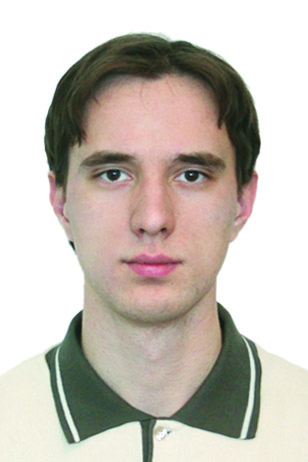
\includegraphics[width=2cm]{photo.jpg}
%    \vspace{-20pt}
%\end{wrapfigure}

    \section{\mysidestyle Contact\\Information}
    Current Location: Los Angeles, United States \\
    Mobile: 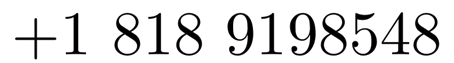
\includegraphics[height=0.35cm]{phone-us.png} \\ 
    E-mail: apfokin@gmail.com 

    %\section{\mysidestyle Personal\\Statement}
    %I strive for excellence in everything that I do. 
    %Software development is my passion, and I take great enjoyment in creating software that has a positive impact on the lives of others. 
    %I like communicating with people and don't shy away from tasks that do not involve writing code, be it helping junior developers to grow professionally or discussing feature requests with a client.

    %I stand out from my peers, even in highly competitive environments. 
    %I was in top 1\% at the university, and currently I'm the most knowledgeable C++/Qt expert at Network Optix.
    %When I came to MSU I was just another student from a small city somewhere in central Russia. At the time of graduation, I was among the top 1\%. 
    %When I have joined Network Optix I was significantly younger than all other members of the team and had much less experience, but I have caught up quickly and soon became the most knowledgeable C++/Qt expert in the company.
    
    %I perform well under pressure. 
    %At Network Optix I have almost single-handedly implemented the first version of the client application in a very limited time, basically making it possible to release the software before an important trade show.

    %I'll be happy to join a team of similarly self-motivated and highly competent professionals in a company with ambitious and far-reaching goals.
    
    %I'm looking for a job in a company that has a visible impact and 
    % a team of similarly self-motivated and highly competent professionals, 
    %I'm looking for a job in an environment where competence 
    
    \section{\mysidestyle Professional\\Experience}
    \textbf{Network Optix, Inc.} \vspace{2mm}\\\vspace{1mm}%
    \textsl{Senior Software Engineer} \hfill \textbf{October 2011 - present}\\ 
	Implemented initial version of the HD Witness client application. Streamlined the UI making it highly intuitive and utilized OpenGL to provide a fluid and visually appealing user experience. Various sources have described HD Witness as the most aesthetically pleasing and user-friendly video management system on the market, which has helped the company to gain a competitive edge.
    
    Currently responsible for development of generic C++ libraries that are used internally, including compile-time reflection for C++ types, data serialization and object-relational mapping. Other responsibilities include design of public APIs and ensuring UI and UX consistency of our desktop and mobile clients.

    
	\textbf{Combild} \vspace{2mm}\\\vspace{1mm}%
	\textsl{Software Development Lead, Co-founder} \hfill \textbf{June 2010 - December 2011}\\	
	Combild was started to create an IT service management (ITSM) system that would target small companies and IT outsourcers, an underserved market niche for which competing solutions such as 1C:ITIL and Itilium were either too expensive or excessively complex. Combild was to offer a lightweight and user-friendly ITSM system with a licensing model specifically targeted at small companies and IT oursourcers.

	%At the time all other solutions on the market were either too bulky and hard to maintain, or were not suitable for the business model of IT outsourcers. Frustrated with the state of things, we have decided to roll out our own product.
	
    My role was to lay out the initial product architecture and to implement the first demonstrable version, and then to work with customers to prioritize and clarify the features and to manage a small development team. 
	%The system was developed in C++/Qt and targeted both Windows and Linux.
    
    %After a year of development we have secured our first customers, but at that point the cash inflow we had wasn't sufficient to cover our expenses. Unable to secure the funding, we had to close the project.

    
    \textbf{Select LTD} \vspace{2mm}\\\vspace{1mm}%
    \textsl{Software Engineer} \hfill \textbf{July 2009 - September 2011}\\
    Was mainly working on SmartDec, a native code decompiler. Laid out the architecture of the decompiler and implemented several frontend and backend plugins, including support for different x86 and PIC assembly input formats. Was responsible for devising novel algorithms that would improve the quality of the decompiled code and would allow for reconstruction of C++-specific constructs. This effort has lead to several publications on international conferences on reverse engineering. Detailed description of the decompiler is available at \url{http://decompilation.info}.
    
    Have also implemented a form recognition toolkit that was subsequently used in some of the Moscow schools for test checking. Detailed description is available at \url{http://elric.ru/wordpress/projects/form-recognition-toolkit/}. 

    Was additionally working on \url{http://mathege.ru}, a national mathematics exam portal developed in Java using Apache Struts web framework. Did both frontend and backend development and have implemented a \LaTeX~to html converter that was used for importing problems into the system.

    
    \textbf{Institute for System Programming of the Russian Academy of Sciences} \vspace{2mm}\\\vspace{1mm}%
    \textsl{Software Engineer} \hfill \textbf{September 2007 - September 2008}\\
    Was working in a team developing a framework for dynamic analysis of binary code. Using C++ metaprogramming techniques implemented a disassembler for MIPS64 architecture that significantly outperformed all other disassemblers for this architecture known to our team.

    \pagebreak    

   
    \textbf{Intel Research Lab at the Moscow State University} \vspace{2mm}\\\vspace{1mm}%
    \textsl{Software Engineering Intern} \hfill \textbf{February 2007 - April 2008}\\
    Was researching computer vision algorithms and have implemented a panorama stitching application. Description is available at \url{https://code.google.com/p/prec/}.

    Was also charged with the development of Ruby bindings for Intel's Integrated Performance Primitives library. Description is available at \url{https://code.google.com/p/ipp4r/}.
    
    
	\textbf{Personal Projects} \vspace{2mm}\\\vspace{1mm}%
    I am an avid programmer and I enjoy writing code in my free time. Throughout the years I have done a lot freelance work and have finished several personal projects, including a real-time ray-tracing engine, a virtual mouse driver for Windows XP, a tool for automatic reconstruction of 3d solids from engineering drawings and a lot of OpenGL demos. For more information check out my Google Code page (\url{https://code.google.com/u/100177180062339664882/}) and my personal website (\url{http://elric.ru/wordpress/projects}).
   
    
    \section{\mysidestyle Education}
    \textbf{Faculty of Computational Mathematics and Cybernetics, Moscow State University}, Moscow, Russia \vspace{2mm}\\\vspace{1mm}%
    \textsl{\ifthenelse{\boolean{foreign}}{Bachelor's}{Specialist} degree in Applied Mathematics and Computer Science} \hfill \textbf{September 2004 - July 2009}\vspace{1mm}\\
    Advisor: Professor Chernov Alexander \\
    Thesis: Reconstruction of Class Hierarchies for Decompilation of C++ Programs \\
    Graduated with high honors. Diploma GPA is 5.0 out of 5.0.

    \textbf{Graduate School of Science and Engineering, Chuo University}, Tokyo, Japan \vspace{2mm}\\\vspace{1mm}%
    \textsl{Full-time non-degree student} \hfill \textbf{September 2008 - March 2009}\vspace{1mm}\\
    Advisor: Professor Mitsunori Makino \\
	Was studying Japanese, working on algorithms for real-time ray tracing and implemented a real-time ray tracer for use with CAVE automatic virtual environment.

%    \section{\mysidestyle Research\\Interests}
%    Image-based modeling and rendering, 3d reconstruction.
%    Ray tracing and global illumination, especially in real time.
%    Software reverse engineering, binary translation, decompilation.

%    \section{\mysidestyle Research\\Experience}
%    \textbf{Select LTD} \vspace{2mm}\\\vspace{1mm}%
%    \hfill \textbf{October 2010 - September 2011}\\
%    I continued my work on C++ decompilation at Select LTD. 

%    \textbf{Institute for System Programming of the Russian Academy of Sciences} \vspace{2mm}\\\vspace{1mm}%
%    \hfill \textbf{July 2008 - September 2010}\\
%    I was doing research on decompilation of C++ programs.


    \section{\mysidestyle Publications}
    A. Fokin, E. Derevenetc, A. Chernov and K. Troshina. ``SmartDec: Approaching C++ Decompilation'',
	in proceedings of the \textsl{18th Working Conference on Reverse Engineering}, pp. 347-356, 2011.
	
	A. Fokin, K. Troshina and A. Chernov. ``Reconstruction of Class Hierarchies for Decompilation of C++ Programs'',
    in proceedings of the \textsl{14th European Conference on Software Maintenance and Reengineering}, pp. 249-252, 2010.

    K. Troshina, A. Chernov and A. Fokin. ``Profile-Based Type Reconstruction for Decompilation'',
    in proceedings of the \textsl{17th International Conference on Program Comprehension}, pp. 263-267, 2009.

    \pagebreak    
    
    \section{\mysidestyle Honours, \\Awards and \\Test Scores}
    TOEFL iBT, 111/120, Moscow, 2010.                                                               \vspace{1mm}\\
    M.V. Lomonosov Scholarship for Academic Excellence, Moscow, 2006-2009.                          \vspace{1mm}\\
    8th Moscow Collegiate Programming Contest, 9th place, Moscow, 2006.                             \vspace{1mm}\\
    7th Moscow Collegiate Programming Contest, 11th place, Moscow, 2005.                            \vspace{1mm}\\
    Unified State Exam in Mathematics, 100/100 (nationwide top), Izhevsk, 2004.                     \vspace{1mm}

    \section{\mysidestyle Professional\\Skills}
    Substantial experience with C++ and Java. \\
	Deep understanding of the underlying principles of modern C++ libraries and frameworks such as Qt and boost. \\
    A lot of experience writing cross-platform C++ code. \\
    Considerable experience with multithreading in C++ and Java. \\
    Knowledge of modern realtime rendering techniques and APIs. \\
	Experience managing a small development team. \\
    Experience with Delphi, x86 Assembly, Linux shell scripting, SQL. \\
    Some experience with C\#, Matlab, Perl and Python.

    \section{\mysidestyle Languages}
    Russian: native \\
    English: fluent \\
    Japanese: intermediate

    \section{\mysidestyle References}
    {\sl Available upon request.}

\end{resume}
\end{document}



















